\chapter{Desenvolvimento do DiaVision}
\label{ch:development}

Neste capítulo são apresentadas as tecnologias utilizadas, as soluções adotadas para os problemas
de acessibilidade identificados no MSL e os resultados alcançados ao final do processo desenvolvimento.

\section{Tecnologias Utilizadas}

Esta seção lista as principais tecnologias e recursos utilizados no desenvolvimento do sistema DiaVision.

\subsection{Visual Studio Code}

O Visual Studio Code (VSCode) é um editor de código \emph{open source} desenvolvido pela Microsoft para Windows, Linux e MacOS.
Ele inclui suporte para depuração, controle de versionamento Git incorporado, realce de sintaxe, IntelliSense
- termo para um conjunto de funcionalidades de edição de código, tais como completar código e informações de parâmetros -
e refatoração de código.

O VSCode também possibilita a instalação de extensões que adicionam funcionalidades ao editor, assim, aumentando a produtividade do desenvolvedor.
Por conta dessas características, esse foi o editor utilizado neste projeto tanto para desenvolver o sistema DiaVision quanto para a parte escrita deste trabalho.

As extensões utilizadas para desenvolvimento da aplicação foram: Flutter e Dart, que dão suporte à criação de aplicações com o SDK do Flutter
e fluttermobx, que oferece atalhos para adicionar componentes de gerenciamento do estado da aplicação. Já Para a parte escrita,
foi utilizado o conjunto de extensões: bibtexLanguage, Code Speell Checker, LaTeX e LaTeX Workshop.

\newpage

\subsection{Github}

O Github é uma plataforma de desenvolvimento e gestão de código-fonte, baseada no Git, que permite aos usuários compartilhar seus projetos e arquivos com controle
de versionamento de código. Com isso é possível realizar \emph{commits}, sendo cada \emph{commit} um ponto de alteração no histórico do
projeto, criar \emph{branches}, ramificações que possibilitam trabalhar em diferentes funcionalidades ao mesmo tempo e realizar \emph{merges},
que é processo de unir ramificações.

O versionamento de código é uma das funcionalidades mais importantes do Git, pois, manter o histórico de alterações
facilita a investigação e resolução de problemas e, em caso de falhas em uma versão do projeto, é possível reverter para uma
versão anterior.

O Github é gratuito e permite a criação de projetos públicos e privados, porém, os repositórios privados possuem limitações
nas funcionalidades da plataforma. Ambos os repositórios, do desenvolvimento do DiaVision\footnote{\url{https://github.com/jnthnklvn/dia_vision}}
e da parte escrita com LaTeX\footnote{\url{https://github.com/jnthnklvn/tcc_dia_vision}} subiram para o GitHub,
inicialmente de forma privada e disponibilizados de forma pública após a finalização deste trabalho.

\subsection{Ambiente de Desenvolvimento}

A máquina principal utilizada para desenvolvimento do sistema DiaVision foi um computador de mesa (do inglês \emph{Desktop}), com o SO Windows 11.
Porém, trata-se do desenvolvimento de uma aplicação multiplataforma e não é possível testar a aplicação para o sistema operacional
iOS, da Apple, em um computador que não seja esteja rodando o macOS. Assim, para validação do aplicativo, também foi
utilizado um MacBook.

O \autoref{qua-esp-maq-gui} mostra as especificações das máquinas utilizadas no desenvolvimento do sistema.

\begin{quadro}[htb!]
    \begin{center}
        \ABNTEXfontereduzida
        \caption{\label{qua-esp-maq-gui}Máquinas de Desenvolvimento.}
        \begin{tabular}{|c|c|c|}
            %\hline
            \hline
                                & \textbf{\emph{Desktop}}  & \textbf{MacBook}        \\
            \hline
            Sistema Operacional & Windows 11 Pro 22H2      & macOS Big Sur 11.3.1    \\
            \hline
            Disco Rígido        & SDD NVMe 512GB e HD 1TB  & 256GB SDD               \\
            \hline
            Memória RAM         & 32GB 3000MHz DDR4        & 8GB 1600MHz DDR3        \\
            \hline
            Processador         & AMD Ryzen 5 5600X 6-Core & Intel Core i5 Dual-Core \\
            \hline
            % \hline
        \end{tabular}
        \legend{Fonte: Autor.}
    \end{center}
\end{quadro}

\newpage

\subsection{Dispositivos de Teste}

Os testes e validações da aplicação, durante o processo de desenvolvimento, foram realizados em dispositivos físicos
rodando o SO Android, porém, para o iOS os testes foram realizados por meio do iOS Simulator, disponível apenas em
computadores com o SO macOS.

Assim, o \autoref{qua-esp-smart} apresenta as especificações dos \emph{smartphones} utilizados durante o desenvolvimento
do aplicativo.

\begin{quadro}[htb!]
    \begin{center}
        \ABNTEXfontereduzida
        \caption{\label{qua-esp-smart}\emph{Smartphones} utilizados no Desenvolvimento.}
        \begin{tabular}{|c|c|c|}
            %\hline
            \hline
                                  & \textbf{Galaxy S20} & \textbf{Redmi Note 8}   \\
            \hline
            Marca                 & Samsung             & Xiaomi                  \\
            \hline
            Sistema Operacional   & Android 12          & Android 9.0             \\
            \hline
            Armazenamento Interno & 128GB               & 32GB                    \\
            \hline
            Memória RAM           & 8GB                 & 3GB                     \\
            \hline
            \emph{Chipset}        & SAMSUNG Exynos 990  & Snapdragon 665 Qualcomm \\
            \hline
            % \hline
        \end{tabular}
        \legend{Fonte: Autor.}
    \end{center}
\end{quadro}

\subsection{Back4app}

O Back4app é uma plataforma gratuita (no plano básico) que segue o modelo de serviço em nuvem \emph{Backend} como Serviço (BaaS, do inglês \emph{Backend as a Service})
para desenvolvimento de \emph{backend} e gerenciamento de infraestrutura com eficiência e facilidade. Com a plataforma é possível
criar estruturas de dados e serviços de forma simples, sem a necessidade de codificação, possibilitando também a adição de código por meio de \emph{Cloud
    Functions}\footnote{Com Funções em Nuvem é possível escrever funções simples que são disparadas a partir de eventos emitidos
    pela infraestrutura e serviços de nuvem.} para criar validações ou funcionalidades mais complexas.

A plataforma é baseada no ParsePlatform, um \emph{framework} de código aberto que fornece um conjunto de SDKs que visam a criação rápida de \emph{backends}
com armazenamentos de objetos e arquivos, autenticação de usuário, \emph{push notifications}, \emph{dashboard} para gerenciamento e integração com aplicações móveis e \emph{web}.

O Back4app também disponibiliza a criação, customização e hospedagem de uma aplicação \emph{web} para administração do sistema.
Sendo possível definir as classes e operações que estarão disponíveis para gerenciamento pelo Administrador do Sistema (ADS).

Devido a simplicidade que o Back4app oferece para criação, gerenciamento e hospedagem de \emph{backend}, comparado
à aplicações convencionais desenvolvidas por meio da codificação, e ao foco deste trabalho, que é o
desenvolvimento da aplicação móvel com o foco na usabilidade, esse foi o serviço escolhido para o desenvolvimento do sistema.

O plano utilizado para o serviço foi o gratuito, que possui limite de 10 mil requisições por mês, 250MB para armazenamento de dados,
1GB para transferência de dados, 1GB para armazenamento de arquivos e 1 \emph{Cloud Code Job}\footnote{\emph{Cloud Jobs} são utilizados
    para execução de funções de longa duração, das quais não é necessário aguardar a resposta, no servidor. Em outras soluções é possível
    executar essas funções periodicamente, porém, essa funcionalidade ainda não está disponível no Back4app e elas precisam ser disparadas
    por meio da API Rest.}.

\subsection{Flutter}

O \emph{framework} escolhido para desenvolvimento do aplicativo móvel foi o Flutter, apresentado no Capítulo \ref{ch:fundament},
devido a sua facilidade no desenvolvimento móvel multiplataforma, possibilitando a geração de aplicações
para Android e iOS a partir de uma base de código única, mantendo desempenho próximo ao de aplicações nativas.

\section{Implementação}

Esta seção detalha as soluções de implementação adotadas, tais como a arquitetura do sistema e as soluções
para os problemas de acessibilidade.

\subsection{Arquitetura}

A estrutura de pastas do projeto está organizada em módulos, os quais não conhecem uns aos outros,
apenas as classes relativas ao próprio módulo estão dentro de cada pasta. A exceção é para os \emph{repositories} (repositórios)
que estão numa camada separada e contém os modelos e as conexões com a fonte de dados.
Essa camada não tem conhecimento a respeito das demais camadas da aplicação.

Dentro de cada módulo estão as outras duas camadas, os \emph{controllers} (controladores) e a \emph{view} (interface visual).
Os \emph{controllers} fazem a mediação entre a \emph{view} e os \emph{repositories}, eles controlam o estado da aplicação,
devendo atualizar a \emph{view} quando receber atualização dos \emph{repositories} e chamar os \emph{repositories}
quando determinados eventos são disparados na \emph{view}.

A \autoref{fig_est_proj} mostra como está organizada essa estrutura de pastas, sendo que a \emph{view}
está divida em \emph{pages}, que são as telas e \emph{widgets}, que são os componentes que fazem parte das telas.

\newpage

\begin{figure}[htb]
    \caption{\label{fig_est_proj}Estrutura de Pastas do Projeto.}
    \begin{center}
        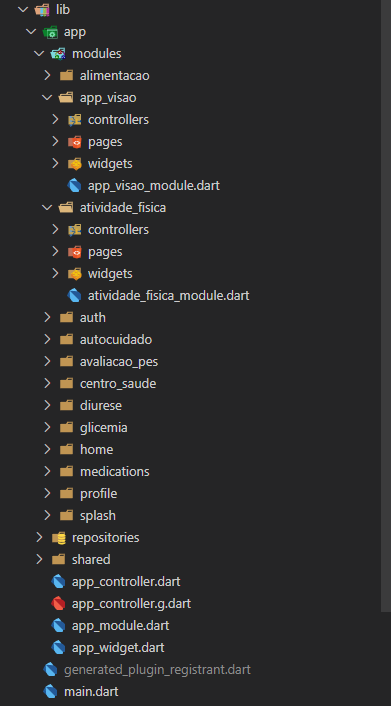
\includegraphics[scale=1]{Imagens/desenvolvimento/arquitetura_dia_vision.png}
    \end{center}
    \legend{Fonte: Autor.}
\end{figure}

Ainda na \autoref{fig_est_proj} percebe-se que dentro de cada módulo existe uma classe geral, é nela onde são definidas
as rotas, injeções de dependências e \emph{singletons}\footnote{\emph{Singleton} é um padrão de projeto que garante
    a existência de apenas uma instância de uma classe.} de cada módulo, como mostra a \autoref{fig_mod_app_vis}.

\newpage

\begin{figure}[htb]
    \caption{\label{fig_mod_app_vis}Classe Principal do Módulo.}
    \begin{center}
        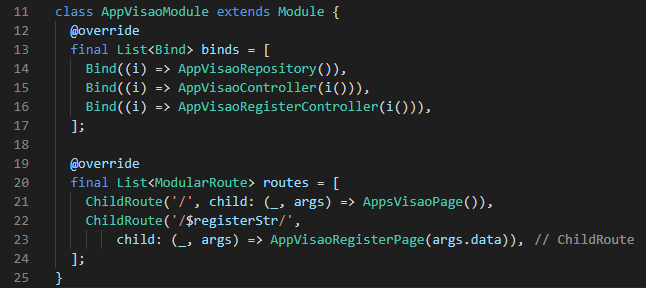
\includegraphics[scale=0.7]{Imagens/desenvolvimento/app_visao_module.png}
    \end{center}
    \legend{Fonte: Autor.}
\end{figure}

Os \emph{singletons} dos repositórios são injetados nos construtores dos controladores como mostrado nas linhas 15
e 16 da \autoref{fig_mod_app_vis} e recuperados pelos controladores conforme mostrado na \autoref{fig_con_app_vis}.

\begin{figure}[htb]
    \caption{\label{fig_con_app_vis}Recuperar Injeção do \emph{Repository} no \emph{Controller}.}
    \begin{center}
        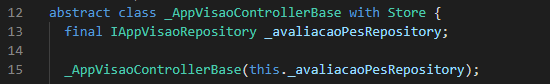
\includegraphics[scale=0.9]{Imagens/desenvolvimento/app_visao_controller.png}
    \end{center}
    \legend{Fonte: Autor.}
\end{figure}

Já os \emph{singletons} dos controladores, por sua vez, são recuperados nas telas,
como nota-se na linha 24 da \autoref{fig_pag_app_vis}.

\begin{figure}[htb]
    \caption{\label{fig_pag_app_vis}Recuperar \emph{Controller} na \emph{Page}.}
    \begin{center}
        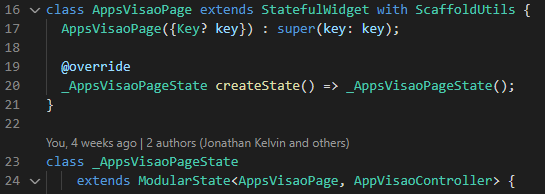
\includegraphics[scale=0.9]{Imagens/desenvolvimento/app_visao_page.png}
    \end{center}
    \legend{Fonte: Autor.}
\end{figure}

\subsection{\emph{Backend}}

O Back4app foi escolhido para o \emph{backend} do sistema e com ele foi possível definir a estrutura de dados, que pode
ser vista na \autoref{fig_bac_app_data}, graficamente por meio de sua interface de usuário.

\begin{figure}[htb]
    \caption{\label{fig_bac_app_data}Esquema do Banco de Dados.}
    \begin{center}
        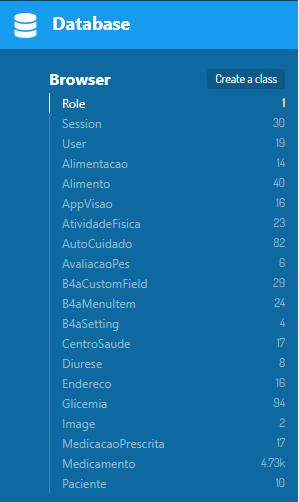
\includegraphics[scale=1.1]{Imagens/desenvolvimento/back4app_database.png}
    \end{center}
    \legend{Fonte: Autor.}
\end{figure}

Embora a plataforma utilize um banco de dados NoSQL - banco de dados não relacional -, o esquema de dados
é definido de forma relacional, onde classes representam tabelas e os relacionamentos são definidos com a utilização
de ponteiros que apontam para objetos de outras classes. Assim, unindo o maior desempenho possibilitado por uma
estrutura NoSQL com uma visão relacional do esquema de dados em alto nível.

\newpage

\subsubsection{Classes do Banco de Dados}

A \autoref{fig_back_data_ali} apresenta a classe ``Alimentacao'' como exemplo, cada classe no banco, por padrão,
possui os atributos objectId, que é utilizado para referenciar os objetos em outras classes por
meio de ponteiros, createdAt, que é a data de criação do objeto, updatedAt, que é a data da última atualização
do objeto, e ACL\footnote{Lista de Controle de Acesso (ACL, do inglês \emph{\textit{Access Control List}})
    são regras de acesso definidas para cada objeto na sua criação.}, que define qual usuário tem permissão de acesso a
esse objeto e quais são essas permissões (escrita, leitura ou ambos).

Com isso, visando a segurança dos dados dos usuários, todas as classes que registram dados dos pessoais
possuem restrição de ACL, onde somente o próprio usuário possui permissão tanto de leitura quanto de escrita.

\begin{figure}[htb]
    \caption{\label{fig_back_data_ali}Exemplo de Classe no Banco.}
    \begin{center}
        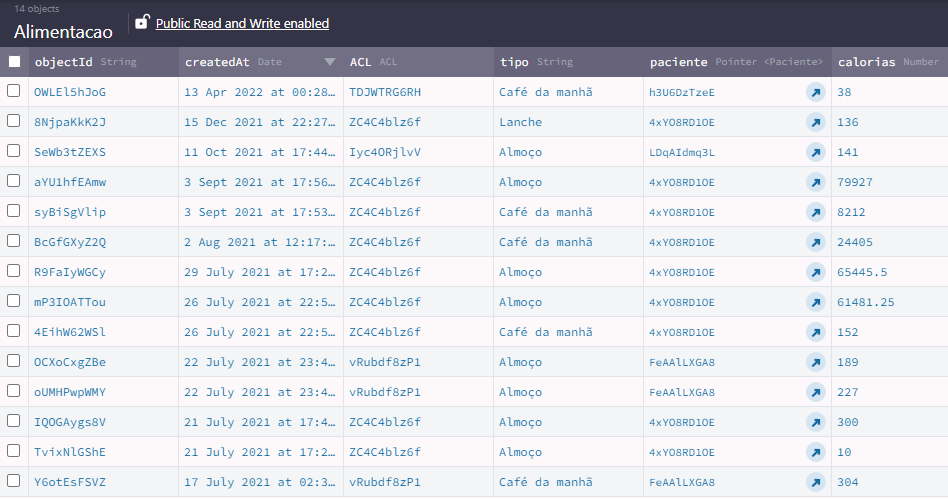
\includegraphics[scale=0.63]{Imagens/desenvolvimento/back4app_database_alimentacao.png}
    \end{center}
    \legend{Fonte: Autor.}
\end{figure}

Ainda na \autoref{fig_back_data_ali}, percebe-se que a classe ``Alimentacao'' possui um atributo chamado paciente do tipo
\emph{Pointer} (Ponteiro) que armazena o objectId que faz referência à classe Paciente como uma chave estrangeira em
bancos de dados relacionais.

\newpage

\subsubsection{\emph{Dashboard} do Administrador do Sistema}

O Back4app também possibilitou a construção de um \emph{dashboard web} para gerenciamento das informações que são disponibilizadas
para os usuários no aplicativo, atendendo aos requisitos funcionais do Administrador do Sistema, mencionados no \autoref{qua-req-fun}.

A customização e disponibilização das funcionalidades nesse \emph{dashboard} foi feita utilizando a própria
interface da plataforma, onde foi possível definir as funcionalidades, campos e perfis acesso que estariam
disponíveis. Ao habilitar o \emph{dashboard} e realizar as customizações, são criadas novas classes no banco
de dados, como pôde ser observado nas que iniciam com "B4a" na \autoref{fig_back_data_ali}, que mantém salvas
essas configurações.

A \autoref{fig_back_dash_auth} apresenta a página de autenticação e a \emph{URL}\footnote{Localizador Uniforme de Recursos
    (URL, do inglês \emph{Uniform Resource Locator}), se refere ao endereço que permite que um site ou recurso seja encontrado na rede.}
de acesso, sendo que as credenciais para autenticar-se são as mesmas utilizadas no aplicativo, porém, com um ACL específico de acesso ao \emph{dashboard}.

\begin{figure}[htb]
    \caption{\label{fig_back_dash_auth}Tela de \emph{Login} do \emph{Dashboard}.}
    \begin{center}
        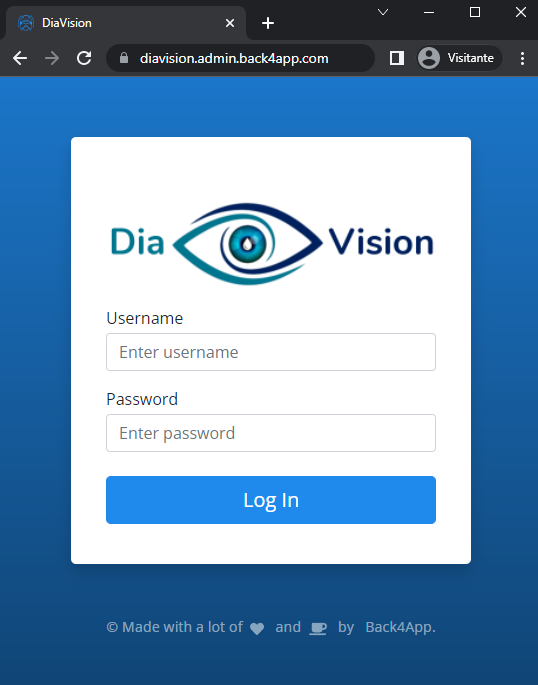
\includegraphics[scale=0.65]{Imagens/desenvolvimento/auth_admin.png}
    \end{center}
    \legend{Fonte: Autor.}
\end{figure}

\newpage

Na \autoref{fig_back_dash_apps} é possível visualizar a tela inicial do \emph{dashboard} com as classes
que estão disponíveis para gerenciamento no menu lateral esquerdo.

\begin{figure}[htb]
    \caption{\label{fig_back_dash_apps}\emph{Dashboard} do Administrador do Sistema.}
    \begin{center}
        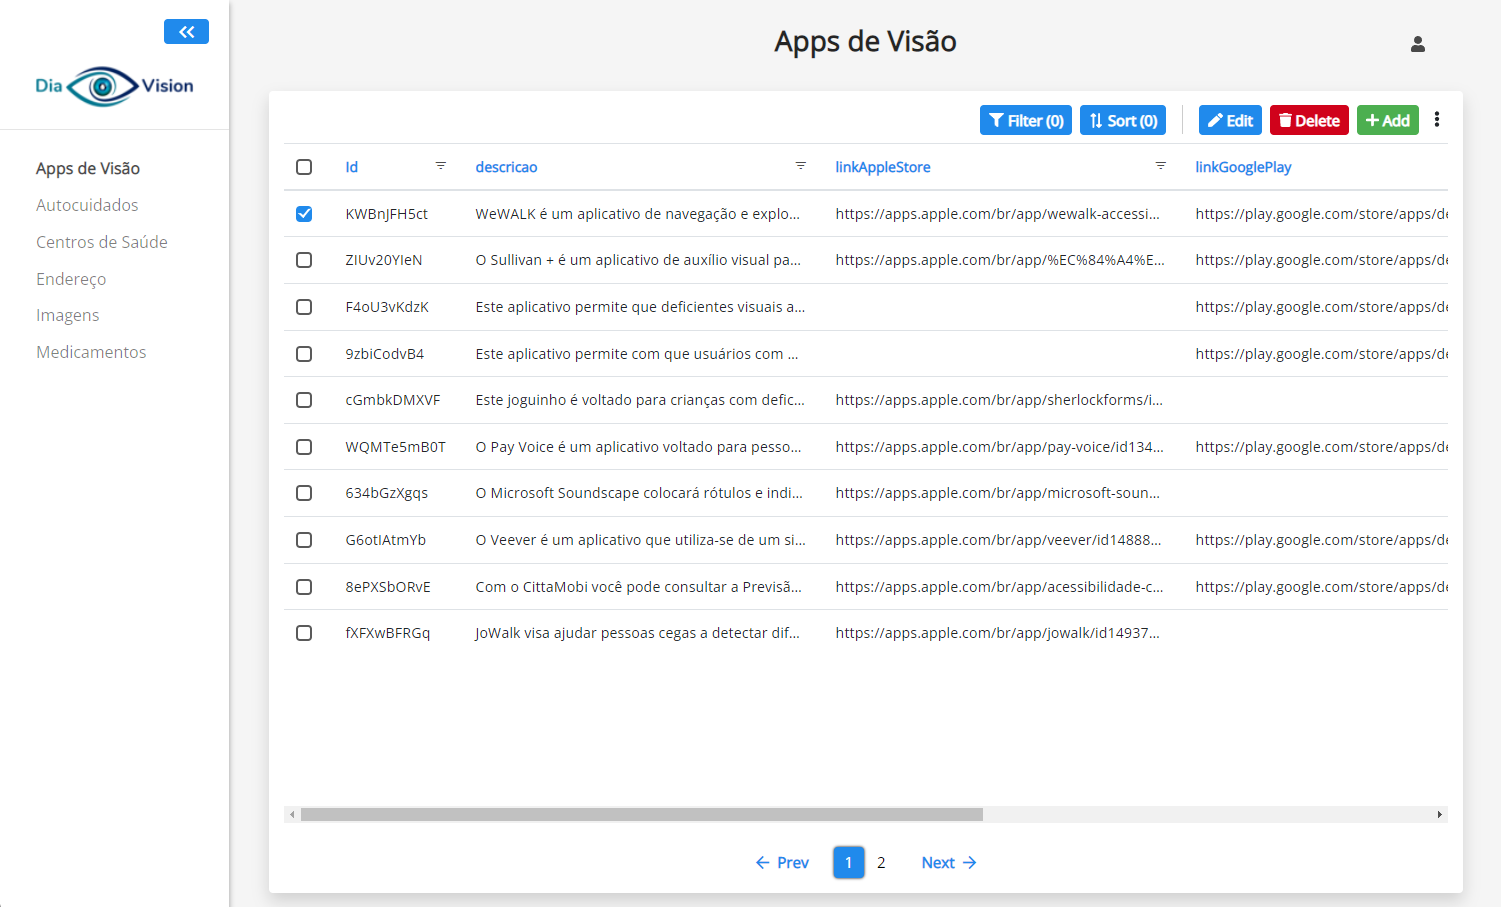
\includegraphics[scale=0.39]{Imagens/desenvolvimento/apps_visao_admin.png}
    \end{center}
    \legend{Fonte: Autor.}
\end{figure}

Assim, a classe ``Apps de Visão'' trata-se de sugestões de aplicativos, de diversas categorias e finalidades, accessíveis
à PDV, essas sugestões podem ser cadastradas pelo ADS ou sugeridas pelos usuários do DiaVision e aprovadas pelo ADS. A
classe ``Centros de Saúde'' segue o mesmo modelo da anterior, porém, se refere à informações sobre centros de saúde, como
nome, descrição, categoria, contatos e endereço.

A classe ``Autocuidados'' armazena dicas de autocuidado com relação à saúde para os usuários. Porém, diferentemente das duas
classes anteriores, apenas o ADS pode cadastrar novas dicas, os usuários do aplicativo não podem criar sugestões.

Já a classe ``Endereço'', armazena as informações de endereços, como nome, rua, CEP etc, e no momento é utilizada apenas
pela classe ``Centro de Saúde''. As imagens com o logotipo do DiaVision exibidas tanto na tela de autenticação quanto na
tela principal do \emph{dashboard} são arquivos cujas referências ficam na classe ``Imagens''.

Por fim, a classe ``Medicamentos'' armazena informações sobre os nomes de medicamentos disponíveis no Brasil, especificamente
o nome de substâncias utilizadas e o nome comercial de cada medicamento. Essas informações são utilizadas para facilitar
o processo para o usuário informar os medicamentos que faz uso no aplicativo DiaVision.

A \autoref{fig_dash_apps_edit} mostra o exemplo de edição de um objeto da classe ``Apps de Visão''. O campo ``verificado''
é utilizado para aprovar as sugestões de \emph{apps} feitas pelos usuários.

\begin{figure}[htb]
    \caption{\label{fig_dash_apps_edit}Página para Edição de Objeto.}
    \begin{center}
        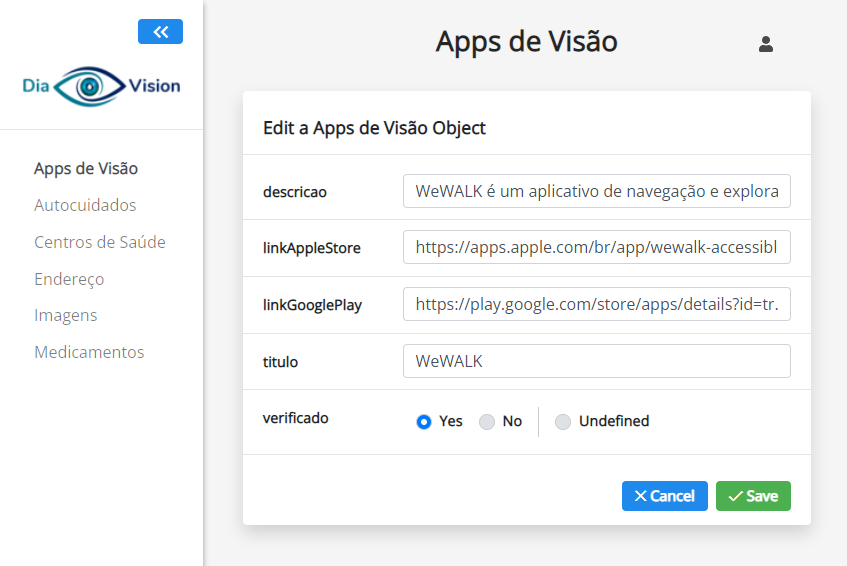
\includegraphics[scale=0.53]{Imagens/desenvolvimento/apps_visao_edit_admin.png}
    \end{center}
    \legend{Fonte: Autor.}
\end{figure}

Na \autoref{fig_dash_auto_add}, pode-se visualizar um exemplo de cadastro do objeto ``Autocuidado''.

\begin{figure}[htb]
    \caption{\label{fig_dash_auto_add}Página para Cadastro de Objeto.}
    \begin{center}
        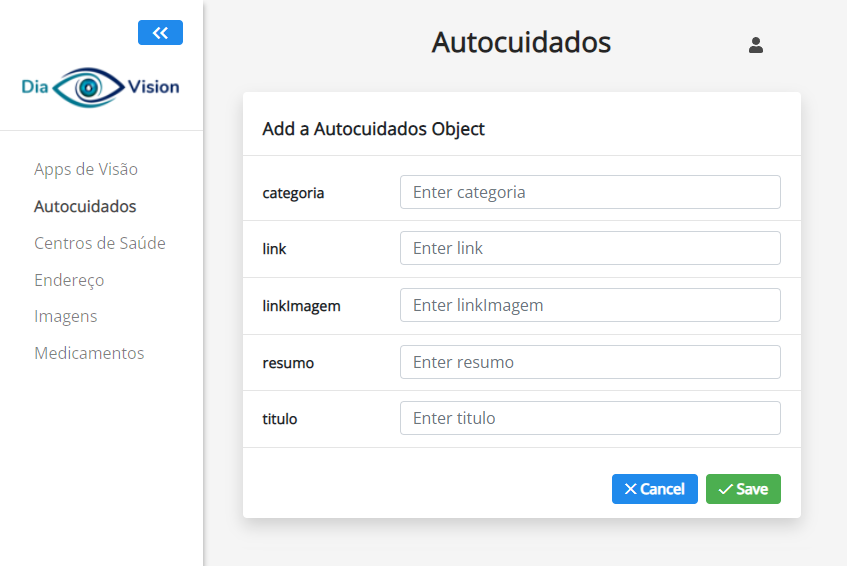
\includegraphics[scale=0.53]{Imagens/desenvolvimento/autocuidados_add_admin.png}
    \end{center}
    \legend{Fonte: Autor.}
\end{figure}

\newpage

\subsection{Aplicativo}

O aplicativo foi desenvolvido utilizando o \emph{framework} de desenvolvimento Flutter, como mencionado
no capitulo anterior, de acordo com os requisitos definidos no planejamento e as soluções de acessibilidade
identificadas no MSL do Capítulo \ref{ch:mapping} e propostas para DiaVision.

\subsubsection{Introdução}

A página inicial do aplicativo pode ser vista na \autoref{fig_app_intro1}, é nela onde é apresentada
uma das principais funcionalidades da aplicação, o \emph{feedback} por voz dos componentes de interface.

\begin{figure}[htb]
    \caption{\label{fig_app_intro1}Introdução ao Aplicativo.}
    \begin{center}
        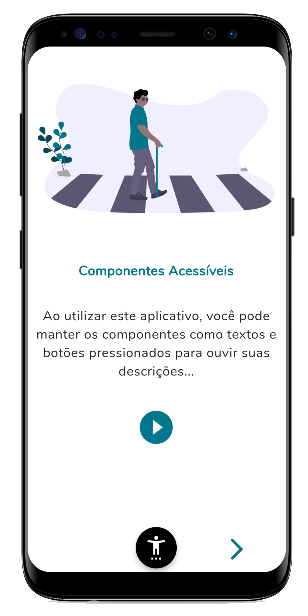
\includegraphics[scale=0.70]{Imagens/desenvolvimento/app/intro_1.png}
    \end{center}
    \legend{Fonte: Autor.}
\end{figure}

Ao pressionar e manter pressionados componentes como botões, textos, imagens etc, uma descrição desses
componentes é lida pelo assistente de voz do aparelho, sem a necessidade de ativar o modo acessibilidade
que habilita os leitores de tela citados no Capítulo \ref{ch:fundament}. Essa funcionalidade faz referência
às soluções de acessibilidade TAM2 e TAM6, propostas para o \emph{app} no final do Capítulo \ref{ch:mapping}.

Ainda na tela inicial, da \autoref{fig_app_intro1}, nota-se que existe um botão flutuante na parte inferior
da tela, a criação dele foi inspirada no AssistiveTouch do iOS\footnote{O AssistiveTouch é um botão flutuante,
    disponível em dispositivos Apple com iOS, que pode ser arrastado para qualquer borda da tela e que abre
    um menu no qual é possível ajustar o volume, bloquear a tela, usar gestos com vários dedos, reiniciar o
    dispositivo etc.}. Já na \autoref{fig_intro_bttn_acs}, o botão flutuante
está em outro canto da tela após ser arrastado para lá pelo usuário.

\begin{figure}[htb]
    \centering
    \begin{minipage}{0.45\textwidth}
        \centering
        \caption{Botão de Acessibilidade.}\label{fig_intro_bttn_acs}
        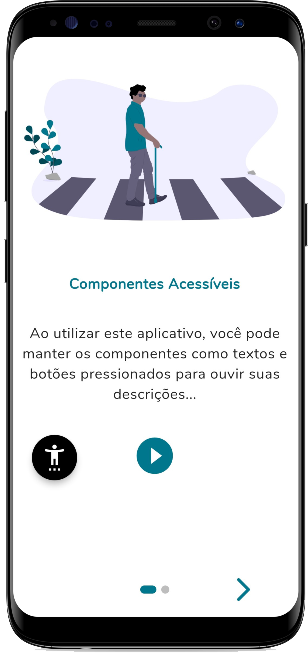
\includegraphics[scale=0.63]{Imagens/desenvolvimento/app/intro_bttn_acs.png}
        \legend{Fonte: Autor.}
    \end{minipage}
    \hfill
    \begin{minipage}{0.45\textwidth}
        \centering
        \caption{Menu de Acessibilidade.}\label{fig_intro_menu_acs}
        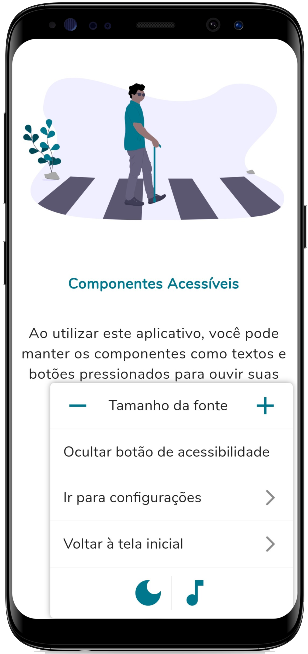
\includegraphics[scale=0.63]{Imagens/desenvolvimento/app/intro_menu_acs.png}
        \legend{Fonte: Autor.}
    \end{minipage}
\end{figure}

Ao clicar no Botão de Acessibilidade, um menu com opções de personalização do aplicativo é aberto,
como pode ser observado na \autoref{fig_intro_menu_acs}. As funcionalidades disponíveis, baseadas nas
soluções de acessibilidade TAM1, TAM4, TAM8 e TAM11, são:

\begin{enumerate}
    \item Aumentar e diminuir o tamanho da fonte de toda a aplicação;
    \item Ocultar o botão de acessibilidade, sendo possível exibi-lo novamente na Tela de Configurações do \emph{app};
    \item Acessar atalhos tanto para a Tela Inicial quanto para a de Configurações do \emph{app};
    \item Alternar o tema do aplicativo entre claro e escuro;
    \item Ativar e desativar o \emph{feedback} por voz de toda a aplicação.
\end{enumerate}

A \autoref{fig_intro_font_inc} exibe o resultado do aumento no tamanho da fonte e da aplicação do tema escuro. Enquanto
na \autoref{fig_app_intro_2} é exibida a segunda tela de introdução, com tema escuro e tamanho normal da fonte,
explicando o funcionamento do botão de acessibilidade para o usuário.

\begin{figure}[htb]
    \centering
    \begin{minipage}{0.47\textwidth}
        \centering
        \caption{Demonstração de Personalização.}\label{fig_intro_font_inc}
        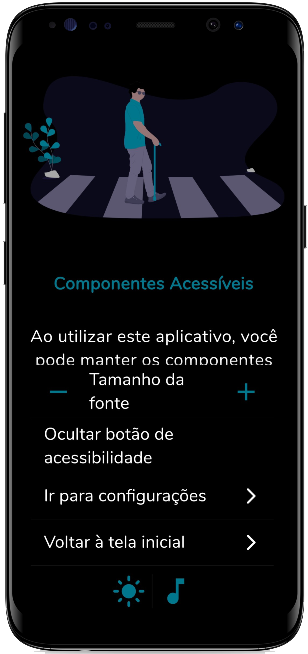
\includegraphics[scale=0.63]{Imagens/desenvolvimento/app/app_intro_font_inc.png}
        \legend{Fonte: Autor.}
    \end{minipage}
    \hfill
    \begin{minipage}{0.44\textwidth}
        \centering
        \caption{Intro Botão de Acessibilidade.}\label{fig_app_intro_2}
        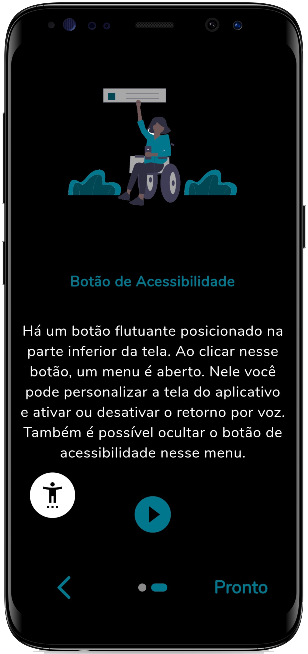
\includegraphics[scale=0.63]{Imagens/desenvolvimento/app/app_intro_2.png}
        \legend{Fonte: Autor.}
    \end{minipage}
\end{figure}

\newpage

\subsubsection{Autenticação}

Ao clicar no botão ``Pronto'', mostrado na \autoref{fig_app_intro_2}, o aplicativo direciona para a tela de autenticação,
apresentada na \autoref{fig_app_login}. A partir dessa tela o usuário pode realizar \emph{login}, informando usuário e
senha, para ser direcionado à tela principal do aplicativo.

\begin{figure}[htb]
    \caption{\label{fig_app_login}Tela de Autenticação.}
    \begin{center}
        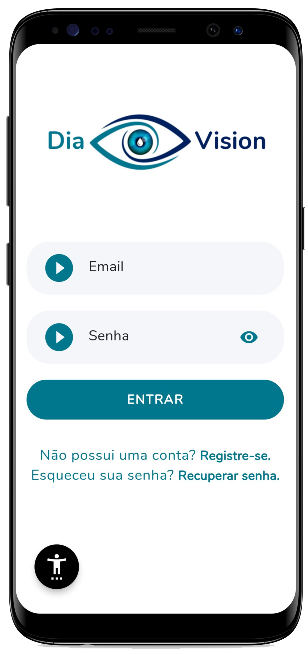
\includegraphics[scale=0.70]{Imagens/desenvolvimento/app/app_login.png}
    \end{center}
    \legend{Fonte: Autor.}
\end{figure}

Além disso, a partir da tela de autenticação também é possível ir para tela de registro,
caso ainda não tenha conta, ou para a tela de recuperação a senha, caso tenha-a esquecido,
clicando nos textos correspondentes abaixo do botão ``Entrar'', este que podê ser visto na
\autoref{fig_app_login}.

\newpage

A tela de registro é apresenta na \autoref{fig_app_register}, nela é possível registrar um novo usuário,
inicialmente, informando apenas e-mail e senha, mas podendo acrescentar mais informações  na tela de Edição
e Dados, após realizar a autenticação.

\begin{figure}[htb]
    \centering
    \begin{minipage}{0.44\textwidth}
        \centering
        \caption{Tela de Registro.}\label{fig_app_register}
        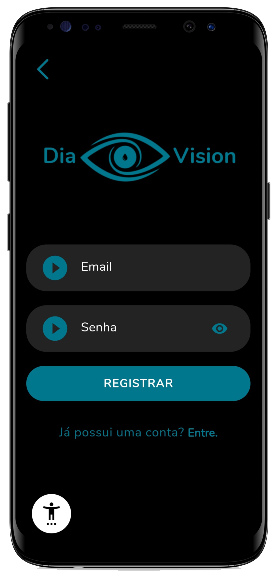
\includegraphics[scale=0.72]{Imagens/desenvolvimento/app/app_register.png}
        \legend{Fonte: Autor.}
    \end{minipage}
    \hfill
    \begin{minipage}{0.47\textwidth}
        \centering
        \caption{Tela para Recuperação de Senha.}\label{fig_app_rec_pass}
        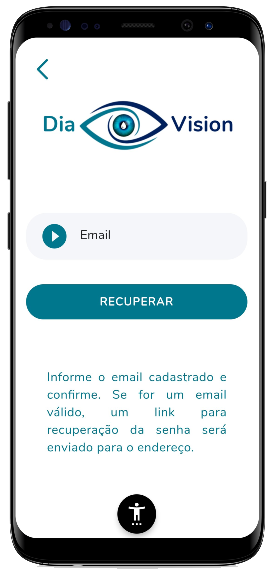
\includegraphics[scale=0.72]{Imagens/desenvolvimento/app/app_rec_pass.png}
        \legend{Fonte: Autor.}
    \end{minipage}
\end{figure}

Já a \autoref{fig_app_rec_pass}, mostra a tela de recuperação de senha, bastando informar o e-mail
da conta para receber um \emph{link} no mesmo endereço para criação da nova senha.

\newpage

\subsubsection{Tela Principal}

A tela principal, é apresentada na \autoref{fig_app_inicio_dark} e na \autoref{fig_app_inicio_2},
é a partir dela que pode-se acessar os módulos e outras funcionalidades do aplicativo.
Na listagem há 9 módulos que podem ser acessados ao clicar em um dos quadrados e, assim
como os demais componentes do \emph{app}, ao mantê-los pressionados, suas descrições
serão lidas pelo assistente de voz do aparelho.

Na primeira imagem o tema está escuro, enquanto que, na segunda, está claro e com o
botão de acessibilidade oculto, mostrando que a personalização da aplicação é dinâmica
e está acessível ao longo de todo o aplicativo.

\begin{figure}[htb]
    \centering
    \begin{minipage}{0.45\textwidth}
        \centering
        \caption{Tela Principal Tema Escuro.}\label{fig_app_inicio_dark}
        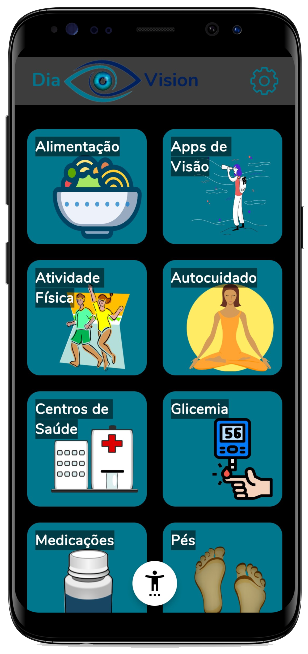
\includegraphics[scale=0.66]{Imagens/desenvolvimento/app/app_inicio_dark.png}
        \legend{Fonte: Autor.}
    \end{minipage}
    \hfill
    \begin{minipage}{0.45\textwidth}
        \centering
        \caption{Restante da Tela Principal.}\label{fig_app_inicio_2}
        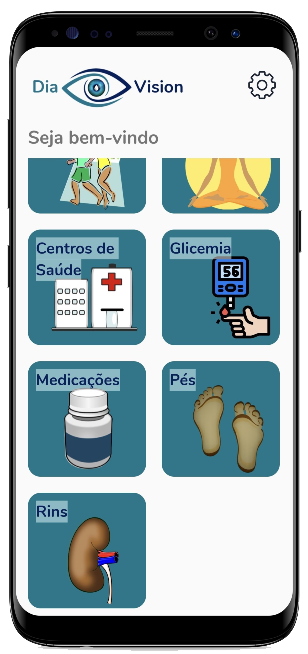
\includegraphics[scale=0.66]{Imagens/desenvolvimento/app/app_inicio_2.png}
        \legend{Fonte: Autor.}
    \end{minipage}
\end{figure}

\subsubsection{Configurações}

O botão de engrenagem no topo da tela principal leva até a tela de configurações, mostrada na
\autoref{fig_app_sett}, onde é possível visualizar e alterar os dados pessoais, editar preferências
e realizar \emph{logoff}.

Na \autoref{fig_app_dat_pref} são apresentadas as telas de edição dos dados do usuário e de preferências.
Em “Meus Dados” o usuário pode alterar os dados de e-mail, nome, telefone, data nascimento, peso e altura.

\begin{figure}[htb]
    \centering
    \begin{minipage}{0.42\textwidth}
        \centering
        \caption{Tela de Configurações.}\label{fig_app_sett}
        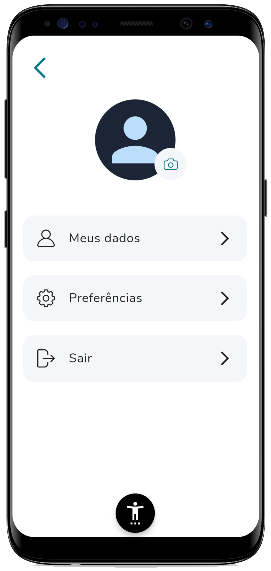
\includegraphics[scale=0.69]{Imagens/desenvolvimento/app/app_sett.png}
        \legend{Fonte: Autor.}
    \end{minipage}
    \hfill
    \begin{minipage}{0.53\textwidth}
        \centering
        \caption{Telas de Preferências e Dados.}\label{fig_app_dat_pref}
        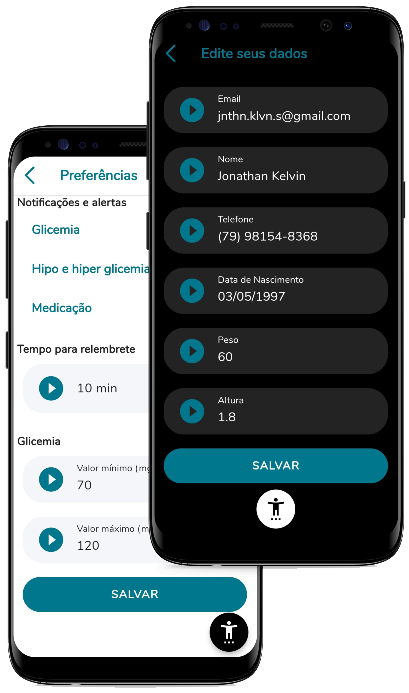
\includegraphics[scale=0.56]{Imagens/desenvolvimento/app/app_dat_pref.png}
        \legend{Fonte: Autor.}
    \end{minipage}
\end{figure}

Já em “Preferências”, como mostrado na \autoref{fig_app_dat_pref}, o usuário pode definir quais notificações
e alertas deseja receber, o tempo para relembrete das notificações e os valores mínimo e máximo de glicemia,
que por padrão são 70 e 120 mg/dL. Bem como, no caso da notificação de glicemia estar ativa, os horários em
que deseja ser lembrado de registrá-la.

\newpage

\subsubsection{Notificações}

As notificações enviadas pelo aplicativo podem ser visualizadas na barra de notificações e possuem um botão
interativo para adiá-las, como mostram a \autoref{fig_app_not_med} e a \autoref{fig_app_not_gli}. Por enquanto,
o tempo adiado se refere ao ``Tempo para relembrete'' definido nas “Preferências”, este que também define
os minutos de antecedência do horário das notificações e registro glicemia.

\begin{figure}[htb]
    \centering
    \begin{minipage}{0.4\textwidth}
        \centering
        \caption{Notificação de Medicação.}\label{fig_app_not_med}
        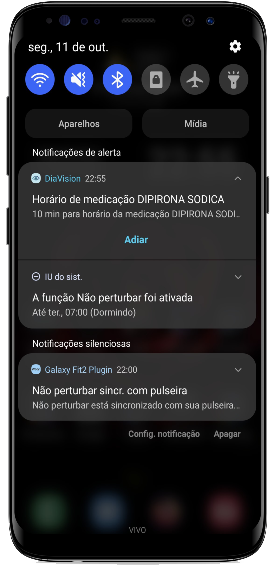
\includegraphics[scale=0.64]{Imagens/desenvolvimento/app/app_not_med.png}
        \legend{Fonte: Autor.}
    \end{minipage}
    \hfill
    \begin{minipage}{0.57\textwidth}
        \centering
        \caption{Notificação de Glicemia.}\label{fig_app_not_gli}
        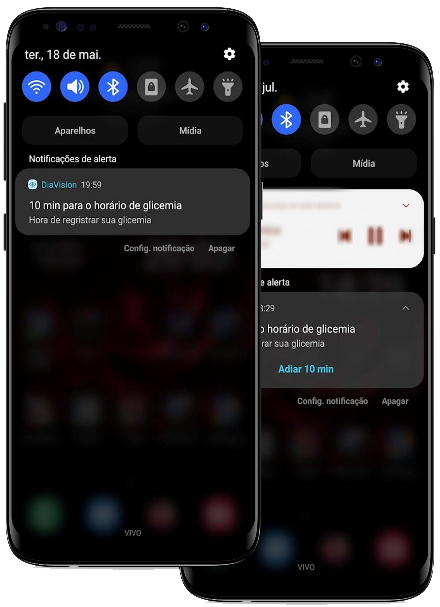
\includegraphics[scale=0.57]{Imagens/desenvolvimento/app/app_not_gli.png}
        \legend{Fonte: Autor.}
    \end{minipage}
\end{figure}

As notificações de medicações são enviadas para lembrar o usuário de que ele precisa tomar uma medicação
nos horários pré-definidos pelo mesmo e para cada medicação. O cadastro de medicações a ativação dessas
notificações será abordado mais à frente.

Já as notificações de glicemia, vistas na \autoref{fig_app_not_gli}, são enviadas periodicamente, também
nos horários definidos pelo usuário, para lembrá-lo de que precisa medir e registrar sua glicemia.

\newpage

\subsubsection{Módulo Alimentacão}

Na primeira tela deste módulo, como pode-se observar na \autoref{fig_list_share_alim}, são listados todos
os registros de alimentação feitos pelo usuário. Também há um botão “compartilhar” no canto superior direito,
por meio do qual é possível exportar esses registros, no formato CSV\footnote{Valores Separados por Vírgula
    (CSV, do inglês \emph{Comma-separated values}) é um formato de arquivo de texto comumente utilizado por
    \emph{softwares} de planilhas como o Google Planilhas, o Microsoft Excel e o \emph{software} livre
    LibreOffice Calc.}, e compartilhá-los para outros \emph{apps}.

\begin{figure}[htb]
    \caption{\label{fig_list_share_alim}Tela Inicial do Módulo Alimentação.}
    \begin{center}
        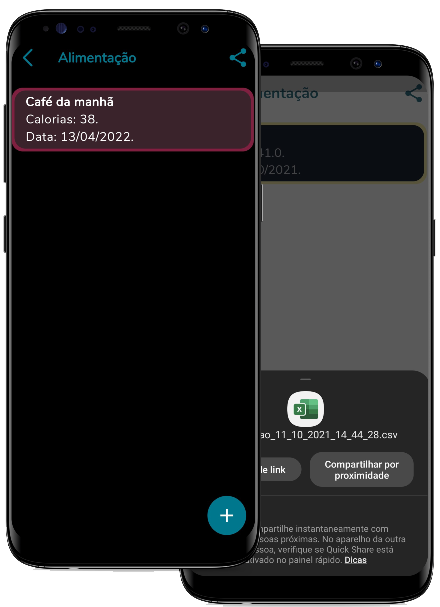
\includegraphics[scale=0.72]{Imagens/desenvolvimento/app/list_share_alim.png}
    \end{center}
    \legend{Fonte: Autor.}
\end{figure}

Ao clicar no botão “+”, no canto inferior direito da \autoref{fig_list_share_alim}, o usuário é direcionado
para a tela de cadastro de alimentação.

Para registrar uma alimentação é necessário definir o tipo (Almoço, Jantar etc) e adicionar cada alimento,
informando as calorias de cada porção consumida. Porém, também é possível não adicionar os alimentos
e informar as calorias totais da refeição diretamente.

A \autoref{fig_reg_alimentacao} mostra a tela de registro de alimentação no estado inicial, sem nenhum alimento
adicionado. A medida que alimentos vão sendo adicionados, esses vão aparecendo na tela e o valor das calorias
também vai sendo atualizado automaticamente com os valores das calorias consumidas de cada alimento, como
observa-se na \autoref{fig_reg_alimentacao_2}.

\begin{figure}[htb]
    \centering
    \begin{minipage}{0.39\textwidth}
        \centering
        \caption{Registro de Alimentação.}\label{fig_reg_alimentacao}
        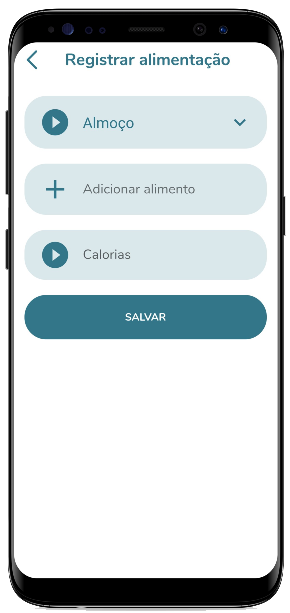
\includegraphics[scale=0.60]{Imagens/desenvolvimento/app/reg_alimentacao.png}
        \legend{Fonte: Autor.}
    \end{minipage}
    \hfill
    \begin{minipage}{0.58\textwidth}
        \centering
        \caption{Adicionando Alimentos.}\label{fig_reg_alimentacao_2}
        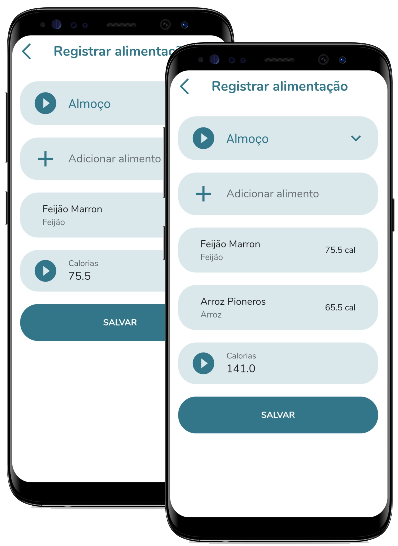
\includegraphics[scale=0.66]{Imagens/desenvolvimento/app/reg_alimentacao_2.png}
        \legend{Fonte: Autor.}
    \end{minipage}
\end{figure}

Para que o cálculo das calorias seja feito automaticamente a cada alimento adicionado, o usuário precisa
informar os dados necessários, sendo estes: nome, porção, calorias por porção e porção consumida. O usuário
não é obrigado a informar nenhum desses dados, porém, caso não informe, o cálculo não poderá ser feito.

\newpage

Cada alimento pode ser adicionado manualmente ou por meio da opção ``Pesquisar alimento...'', localizada
na barra superior do aplicativo na \autoref{fig_reg_alimento}, na qual o usuário
informa o nome do alimento ou parte dele e o \emph{app} faz uma busca pelo alimento referido.

\begin{figure}[htb]
    \centering
    \begin{minipage}{0.39\textwidth}
        \centering
        \caption{Registro de Alimento.}\label{fig_reg_alimento}
        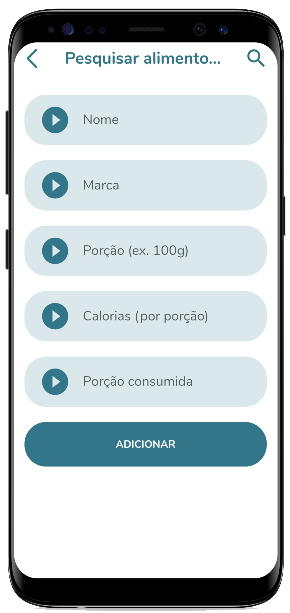
\includegraphics[scale=0.59]{Imagens/desenvolvimento/app/reg_alimento.png}
        \legend{Fonte: Autor.}
    \end{minipage}
    \hfill
    \begin{minipage}{0.58\textwidth}
        \centering
        \caption{Buscar Alimento.}\label{fig_busca_alimento}
        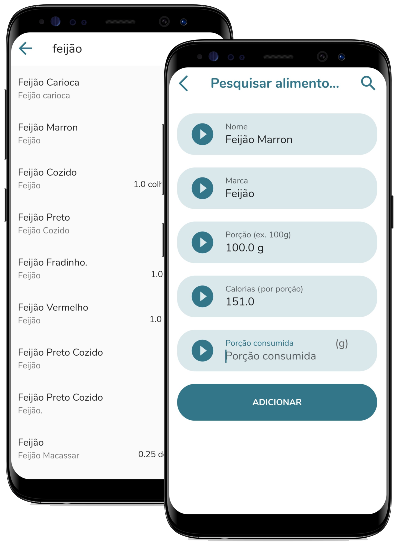
\includegraphics[scale=0.66]{Imagens/desenvolvimento/app/busca_alimento.png}
        \legend{Fonte: Autor.}
    \end{minipage}
\end{figure}

Ao realizar a busca, o \emph{app} retorna uma lista de alimentos que possuem os nomes parecidos com o
informado, como nota-se na \autoref{fig_busca_alimento}. Os alimentos são retornados com os valores de
porção, unidade de medida e calorias por porção, assim, ao selecionar um desses alimentos, resta ao usuário
apenas informar a quantidade consumida na mesma unidade indicada para o alimento selecionado.

\newpage

\subsubsection{Módulo \emph{Apps} de Visão}

Neste módulo, são apresentados sugestões de aplicativos de diversos temas que auxiliam, de alguma forma, pessoas
com deficiência visual, como constata-se na \autoref{fig_list_apps_visao}. Ao clicar em um deles, o usuário será
direcionado à página do \emph{app} na loja de aplicativos, de acordo com SO do \emph{smartphone} utilizado.

\begin{figure}[htb]
    \centering
    \begin{minipage}{0.45\textwidth}
        \centering
        \caption{Listagem de \emph{Apps} de Visão.}\label{fig_list_apps_visao}
        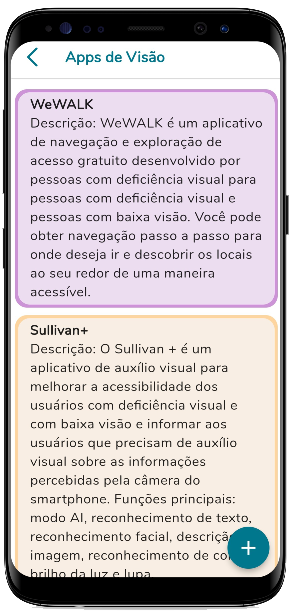
\includegraphics[scale=0.66]{Imagens/desenvolvimento/app/list_apps_visao.png}
        \legend{Fonte: Autor.}
    \end{minipage}
    \hfill
    \begin{minipage}{0.45\textwidth}
        \centering
        \caption{Sugerir \emph{App} de Visão.}\label{fig_sug_apps_visao}
        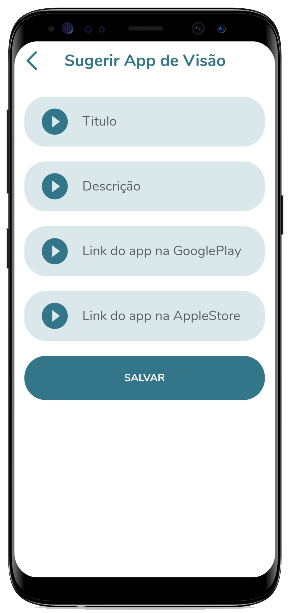
\includegraphics[scale=0.66]{Imagens/desenvolvimento/app/sug_apps_visao.png}
        \legend{Fonte: Autor.}
    \end{minipage}
\end{figure}

Vale ressaltar que as sugestões podem ser diferentes de acordo com o SO, caso um \emph{app} esteja disponível
apenas para Android, não aparecerá na listagem ao acessar esse módulo em um dispositivo iOS e vice-versa.

O usuário também pode sugerir algum aplicativo que acredite ser útil para pessoas com deficiência visual, como
visto na \autoref{fig_sug_apps_visao}. As sugestões recebidas são aprovadas por um administrador do sistema, se
estiverem de acordo com o esperado.

\subsubsection{Módulo Atividade Física}

Este módulo tem o objetivo de oferecer uma opção para gerenciamento das atividades físicas praticadas
pelo usuário. Nesta tela inicial há uma listagem simples dos exercícios físicos registrados, como mostra a
\autoref{fig_list_atv_fis}. Ao clicar em um deles, o usuário é direcionado a página de edição da atividade,
para que possa alterar algum dado informado.

\begin{figure}[htb]
    \centering
    \begin{minipage}{0.45\textwidth}
        \centering
        \caption{Listagem de Atividades Física.}\label{fig_list_atv_fis}
        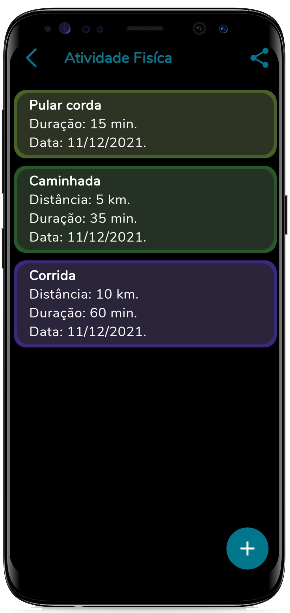
\includegraphics[scale=0.66]{Imagens/desenvolvimento/app/list_atv_fis.png}
        \legend{Fonte: Autor.}
    \end{minipage}
    \hfill
    \begin{minipage}{0.45\textwidth}
        \centering
        \caption{Registro de Atividade Física.}\label{fig_reg_atv_fis}
        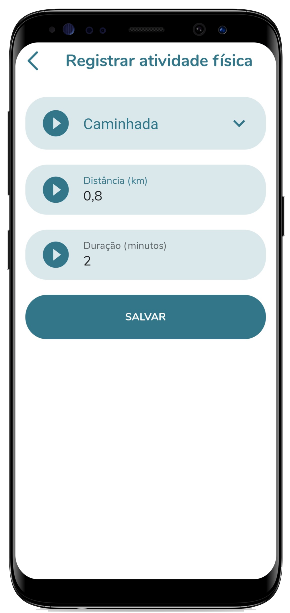
\includegraphics[scale=0.66]{Imagens/desenvolvimento/app/reg_atv_fis.png}
        \legend{Fonte: Autor.}
    \end{minipage}
\end{figure}

Por enquanto pode-se registrar apenas exercícios considerando o tempo que foi praticado e a distância, sendo
que, esta última se aplica somente nos dois tipos predefinidos (caminhada e corrida). Neste módulo também há a
opção de compartilhar os registros no formato CSV\@.

Para o registro mostrado na \autoref{fig_reg_atv_fis}, o primeiro campo solicitado é o tipo, que pode ser um
dos predefinidos ou “Outro”, este que pode ser informado pelo usuário no campo que surge quando essa opção é
selecionada. O segundo campo varia de acordo com a opção selecionada no primeiro. E o terceiro é a duração,
em minutos, do exercício.

\subsubsection{Módulo Autocuidado}

Na tela inicial deste módulo, como mostra a \autoref{fig_list_autoc}, são listadas dicas de autocuidado
divididas em diversas categorias, onde o usuário pode filtrar por alguma específica ou manter todas as
categorias na listagem.

Essas dicas são cadastradas, exclusivamente, por um administrador do sistema de acordo com recomendações
validadas por profissionais da saúde.

\begin{figure}[htb]
    \centering
    \begin{minipage}{0.5\textwidth}
        \centering
        \caption{Listagem de Autocuidados.}\label{fig_list_autoc}
        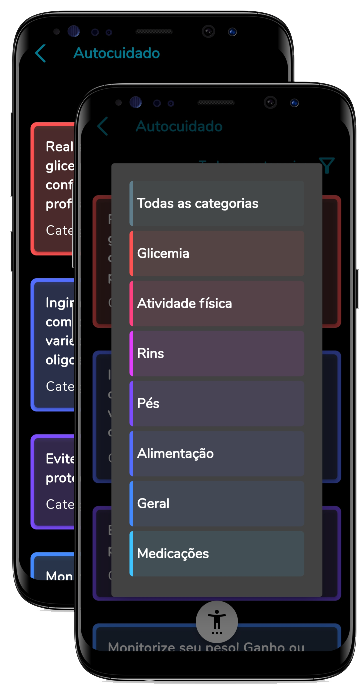
\includegraphics[scale=0.6]{Imagens/desenvolvimento/app/list_autoc.png}
        \legend{Fonte: Autor.}
    \end{minipage}
    \hfill
    \begin{minipage}{0.45\textwidth}
        \centering
        \caption{Tela de Autocuidado.}\label{fig_page_autoc}
        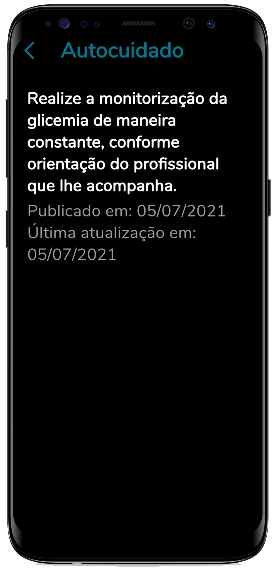
\includegraphics[scale=0.72]{Imagens/desenvolvimento/app/page_autoc.png}
        \legend{Fonte: Autor.}
    \end{minipage}
\end{figure}

Ao clicar em um dos componentes de autocuidado, é aberta uma nova tela com os detalhes. Essa tela pode
conter título, descrição e as datas de publicação e última atualização da dica, como foi mostrado na
\autoref{fig_page_autoc}.

\subsubsection{Módulo Centros de Saúde}

Neste módulo são listados, na tela principal, centros de saúde com informações sobre o tipo, nome, descrição,
telefones para contato, endereço e localização no Google Maps\footnote{O Google Maps é um serviço de busca e
    visualizar de mapas, localizações e rotas oferecido pelo Google de forma gratuita.}.

Como pode-se observar na \autoref{fig_list_centros}, a listagem possui uma filtragem por tipo, assim,
em conjunto com às funcionalidades de acessibilidade do \emph{app}, o usuário pode encontrar por
centros de saúde que atendam sua demanda de maneira mais acessível.

\begin{figure}[htb]
    \centering
    \begin{minipage}{0.5\textwidth}
        \centering
        \caption{Listagem de Centros de Saúde.}\label{fig_list_centros}
        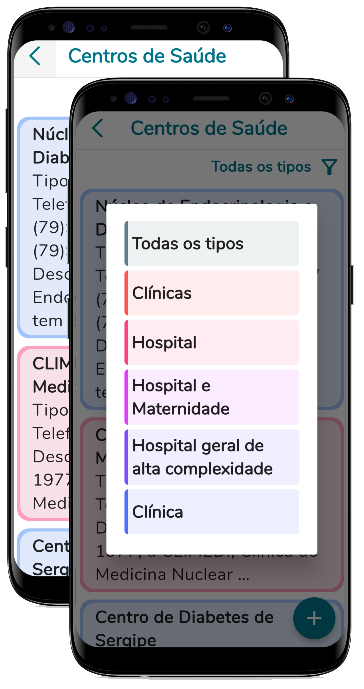
\includegraphics[scale=0.6]{Imagens/desenvolvimento/app/list_centros.png}
        \legend{Fonte: Autor.}
    \end{minipage}
    \hfill
    \begin{minipage}{0.45\textwidth}
        \centering
        \caption{Tela do Centro de Saúde.}\label{fig_page_centro}
        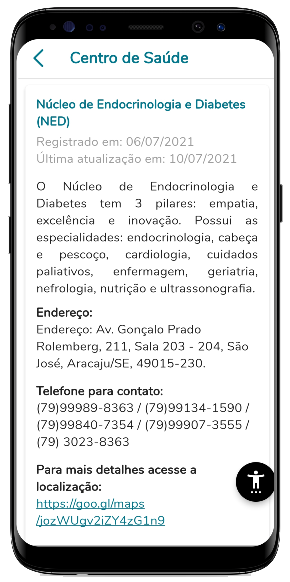
\includegraphics[scale=0.7]{Imagens/desenvolvimento/app/page_centro.png}
        \legend{Fonte: Autor.}
    \end{minipage}
\end{figure}

Ao clicar em um dos componentes de centro de saúde, o usuário é direcionado para uma tela como a da
\autoref{fig_page_centro}, na qual ele pode visualizar os detalhes desse centro.

Além disso, o usuário também pode sugerir novos centros de saúde para o sistema, funcionando da mesma forma das
sugestões de \emph{apps} de visão.

\subsubsection{Módulo Glicemia}

Na tela inicial do módulo de glicemia é exibida uma listagem dos registros de glicemia feitos pelo usuário.
Esses registros também podem ser exportados da mesma forma que os registros de alimentação e atividade física.

Ao clicar no botão “+” no fim da tela mostrada na \autoref{fig_list_glicemia}, é possível inserir um novo registro. Porém, na primeira vez que o botão
é pressionado, um dialogo é exibido perguntando se o usuário quer manter os limites padrões de glicemia ou
definir os próprios, como mostra a figura.

\begin{figure}[htb]
    \centering
    \begin{minipage}{0.5\textwidth}
        \centering
        \caption{Listagem de Registros de Glicemia.}\label{fig_list_glicemia}
        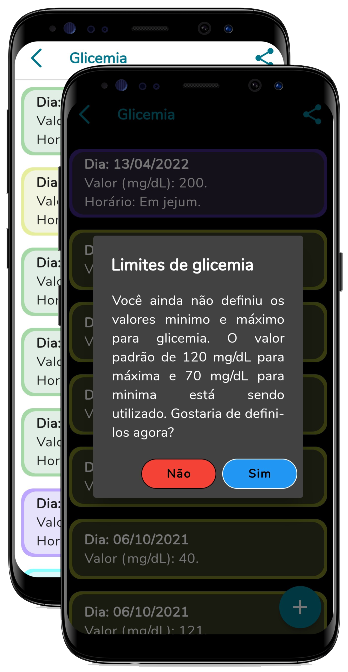
\includegraphics[scale=0.6]{Imagens/desenvolvimento/app/list_glicemia.png}
        \legend{Fonte: Autor.}
    \end{minipage}
    \hfill
    \begin{minipage}{0.45\textwidth}
        \centering
        \caption{Alerta de Glicemia.}\label{fig_alerta_glicemia}
        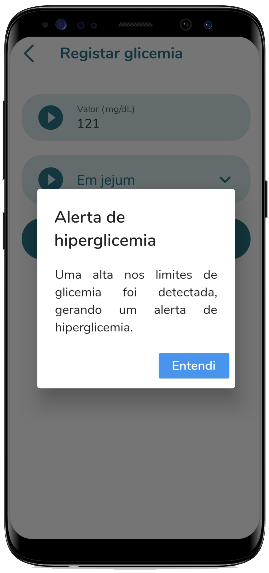
\includegraphics[scale=0.7]{Imagens/desenvolvimento/app/alerta_glicemia.png}
        \legend{Fonte: Autor.}
    \end{minipage}
\end{figure}

Ao registrar um valor de glicemia, caso ele seja superior ao limite máximo ou inferior ao mínimo,
um alerta de hiper ou hipoglicemia, respectivamente, será exibido, de acordo com os valores definidos
nas “Preferências”.

\subsubsection{Módulo Medicações}

O objetivo geral deste módulo é que o usuário registre todas as medicações que faz uso para que possa ser
notificado alguns minutos antes de cada horário de medicação.

Assim, como mostra a \autoref{fig_list_med}, na primeira tela do módulo são listadas as medicações que o usuário
registrou. Para cada uma dessas medicações, é exibido um botão para ativar as notificações, caso ele esteja verde,
as notificações para essa medicação estão desativadas, e ativadas caso contrário, como pode ser visto
na \autoref{fig_list_med_not}.

É importante ressaltar que o \emph{feedback} por voz da aplicação, caso esteja ativo, se aplica também à
mensagens de alerta como a exibida na \autoref{fig_list_med_not}.

\begin{figure}[htb]
    \centering
    \begin{minipage}{0.45\textwidth}
        \centering
        \caption{Listagem de Medicações.}\label{fig_list_med}
        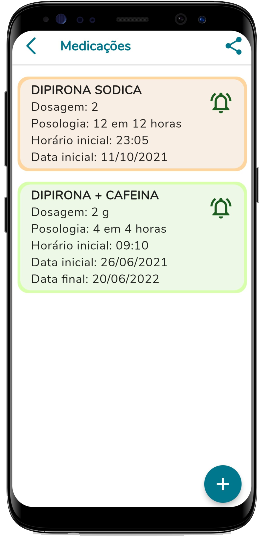
\includegraphics[scale=0.66]{Imagens/desenvolvimento/app/list_med.png}
        \legend{Fonte: Autor.}
    \end{minipage}
    \hfill
    \begin{minipage}{0.45\textwidth}
        \centering
        \caption{Notificar de Medicação.}\label{fig_list_med_not}
        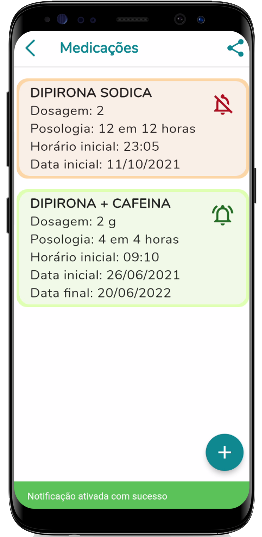
\includegraphics[scale=0.66]{Imagens/desenvolvimento/app/list_med_not.png}
        \legend{Fonte: Autor.}
    \end{minipage}
\end{figure}

As notificações de medicações são baseadas no horário inicial e na posologia, e aparecem determinado tempo
antes de cada horário, sendo 10 minutos por padrão e podendo ser alterado nas “Preferências”.

Para registro de medicação, alguns dados como nome, dosagem, posologia, horário inicial e data final,
são importantes para que o usuário possa ser notificado. Isso porque a posologia (intervalo entre as doses)
e o horário inicial definem os horários de notificação. A data final define quando as notificações devem
parar. E, o nome e a dosagem são exibidos na notificação de lembrete.

Porém, nenhum desses dados, exibidos na \autoref{fig_reg_med}, são obrigatórios. Assim, se não informados,
o usuário não será notificado nos horários que deve tomar as medicações.

\begin{figure}[htb]
    \centering
    \begin{minipage}{0.45\textwidth}
        \centering
        \caption{Registro de Medicação.}\label{fig_reg_med}
        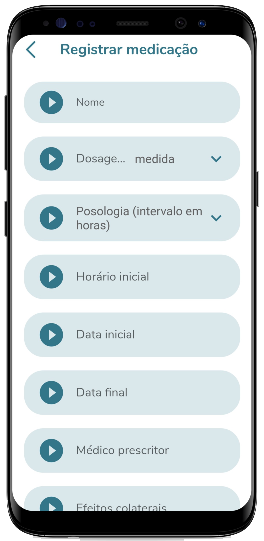
\includegraphics[scale=0.66]{Imagens/desenvolvimento/app/reg_med.png}
        \legend{Fonte: Autor.}
    \end{minipage}
    \hfill
    \begin{minipage}{0.46\textwidth}
        \centering
        \caption{\emph{Autocomplete} de Medicamentos.}\label{fig_reg_med_auto_comp}
        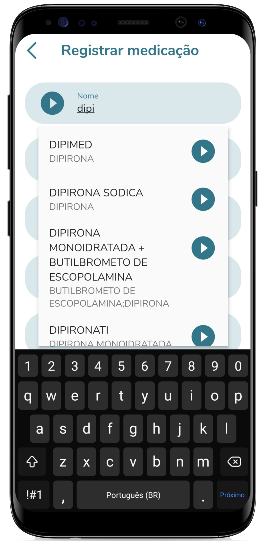
\includegraphics[scale=0.66]{Imagens/desenvolvimento/app/reg_med_auto_comp.png}
        \legend{Fonte: Autor.}
    \end{minipage}
\end{figure}

Ao digitar o nome da medicação no campo “Nome”, após a quarta letra, o \emph{app} começa a buscar e filtrar
sugestões para a medicação que está sendo buscada, como mostra o exemplo na \autoref{fig_reg_med_auto_comp}.

Contudo, nessa listagem de sugestões, diferente da maioria dos componentes do aplicativo, não é possível ouvir o
\emph{feedback} com as descrições ao manter os itens pressionados. Isso ocorre devido a uma limitação do
componente utilizado e por esta razão existe o ``ícone de \emph{play}'' ao lado de cada item para cumprir
esse papel.

\subsubsection{Módulo Pés}

Este módulo serve para que o usuário possa acompanhar a evolução dos cuidados com os pés, com o registro
diário de avaliação do estado dos mesmos.

Como nos demais módulos de registros pessoais do usuário, no canto superior direito da \autoref{fig_list_ava_pes}
tem um botão para compartilhar esses registros. Assim, o usuário pode utilizar esse recurso para compartilhar as
avaliações com seu podologista ou com algum familiar responsável por acompanhá-lo na visita ao profissional.

\begin{figure}[htb]
    \centering
    \begin{minipage}{0.47\textwidth}
        \centering
        \caption{Listagem de Avaliações dos Pés.}\label{fig_list_ava_pes}
        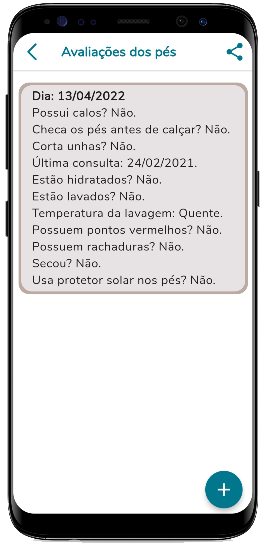
\includegraphics[scale=0.66]{Imagens/desenvolvimento/app/list_ava_pes.png}
        \legend{Fonte: Autor.}
    \end{minipage}
    \hfill
    \begin{minipage}{0.45\textwidth}
        \centering
        \caption{Avaliar Pés.}\label{fig_reg_ava_pes}
        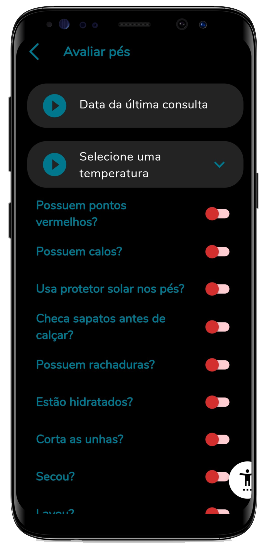
\includegraphics[scale=0.66]{Imagens/desenvolvimento/app/reg_ava_pes.png}
        \legend{Fonte: Autor.}
    \end{minipage}
\end{figure}

No registro de avaliação, o usuário pode informar a data da última consulta e a temperatura da água utilizada
para lavagem dos pés. Além disso, há várias perguntas de “Sim” ou “Não” com detalhes que podem descrever o
estado dos pés do usuário em cada registro, como mostrou a \autoref{fig_reg_ava_pes}.

\subsubsection{Módulo Rins}

Este é o último módulo e se refere ao acompanhamento dos rins e diurese - quantidade de urina produzida em
determinado período -, listando os registros diários de diurese na tela inicial como pode-se observar na
\autoref{fig_list_diurese}.

Essas informações podem auxiliar o usuário na visita ao profissional da saúde, pois, oferecem dados que
possibilitam a avaliação da função renal. Assim, também há a funcionalidade para compartilhamento desses
registros.

\begin{figure}[htb]
    \centering
    \begin{minipage}{0.47\textwidth}
        \centering
        \caption{Listagem de Diurese.}\label{fig_list_diurese}
        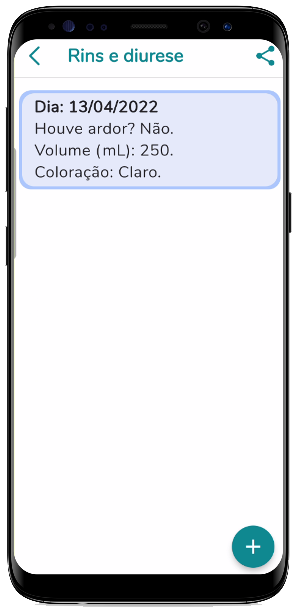
\includegraphics[scale=0.66]{Imagens/desenvolvimento/app/list_diurese.png}
        \legend{Fonte: Autor.}
    \end{minipage}
    \hfill
    \begin{minipage}{0.45\textwidth}
        \centering
        \caption{Avaliar Diurese.}\label{fig_reg_diurese}
        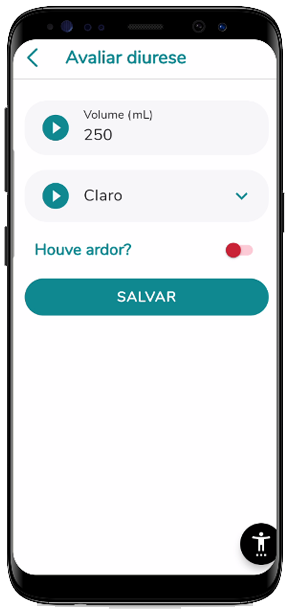
\includegraphics[scale=0.66]{Imagens/desenvolvimento/app/reg_diurese.png}
        \legend{Fonte: Autor.}
    \end{minipage}
\end{figure}

Na avaliação de diurese, conforme mostrado na \autoref{fig_reg_diurese}, são solicitados o volume em mL
(mililitros), uma avaliação da coloração da urina e se houve ardor.

Como esses registros sempre acrescentam a data automaticamente, o usuário pode fazer o registro
a cada vez que urina ou somente uma vez somando todo o volume diário. A estratégia fica a cargo do usuário,
devendo o mesmo relatar o método utilizado para o profissional responsável.

\section{Considerações Finais}

Este capítulo buscou elucidar o processo de desenvolvimento, relatando a estrutura do projeto, as tecnologias
utilizadas, as soluções de acessibilidade adotas e o resultado final do sistema DiaVision. Este que incluiu o
aplicativo móvel multiplataforma e a aplicação \emph{backend} para gerenciamento dos dados, que também ofereceu
suporte para criação de um \emph{dashboard} para administração de dados do sistema.